\begin{frame}{Appendix}{Challenges in Defining Constraint Guides (RAG, RRG, GRG)}

\textbf{Problem:} Defining constraint guides in MARL is challenging in practice.

\begin{itemize}
  \item A full specification "by extension" is impractical:
    \begin{itemize}
      \item Enumerating all possible observation or history cases is intractable.
      \item Maintaining and updating such rules does not scale.
    \end{itemize}

  \item \textbf{We propose two intensional strategies to define constraint guides:}
  \begin{enumerate}
    \item \textbf{Custom logic scripting:} Users define Python functions (per role/goal) that take in trajectory and observation to return:
    \begin{itemize}
      \item RAG: allowed actions with hardness weights
      \item RRG: reward penalties/bonuses for specific actions
      \item GRG: reward shaping based on trajectory features
    \end{itemize}
    \item \textbf{Trajectory Patterns (TPs):} Compact, declarative patterns inspired by NLP to match a set of trajectories to represent a behavior.
  \end{enumerate}
\end{itemize}

\end{frame}

%==================================================

\begin{frame}{Appendix}{Solution 1: Constraint Guides via Custom Scripting}

\textbf{Principle:} Define a function per role/goal that analyzes trajectory and current observation.

\vspace{0.5em}
\textbf{Example (Overcooked-AI)}:

\begin{itemize}
  \item \textbf{Role: Primary cook}
  \item \textbf{Observation:} Agent is holding a dish, a pot is ready, no wall ahead
  \item \textbf{Trajectory:} Previously picked onion, then chopped
\end{itemize}

\textbf{Script outputs:}

\begin{itemize}
  \item \textbf{RAG:} \{`interact' $\rightarrow$ 1.0, `nothing' $\rightarrow$ 0.2\}
  \item \textbf{RRG:} +2 bonus if `interact' is used near ready pot
  \item \textbf{GRG:} +1 if trajectory ends with delivery of soup
\end{itemize}

\textbf{Advantage:} Custom logic can consider spatial layout, previous steps, object held, etc.

\end{frame}

%==================================================

\begin{frame}{Appendix}{Solution 2: Constraint Guides via Trajectory Patterns (TPs)}

\textbf{Principle:} Define reusable and human-readable trajectory patterns to match agent behavior.

\vspace{0.5em}
\textbf{Format:} TP = pattern transitions as \textbf{\textit{[obs, act | sub\_TP]($n_{min}$, $n_{max}$)}}

\textbf{Example (Overcooked-AI):}

\begin{itemize}
  \item \textbf{Pattern:} \\ \textit{[`see\_onion`, `interact`, [\#any](*),`see\_chopped`, `interact`, [\#any](*), `see\_pot`, `interact`](1,1)}
  \item \textbf{TP Match:} Agent has filled pot with chopped onion
  \item \textbf{Current Observation:} \texttt{see\_ready\_pot}
\end{itemize}

\textbf{Then:}
\begin{itemize}
  \item \textbf{RAG:} Only allow `interact`
  \item \textbf{RRG:} +3 bonus for `interact` now
  \item \textbf{GRG:} Encourage reaching delivery window afterward
\end{itemize}

\textbf{Benefits:}
\begin{itemize}
  \item Easier to define symbolic patterns across different environments
  \item Compact encoding of temporally extended behavior
  \item TPs can be reused across agents and roles
\end{itemize}

\end{frame}

\begin{frame}{Appendix}{Software and hardware configuration}

  \begin{block}{MMA – MOISE+MARL API}
    \begin{itemize}
      \item Python API integrating:
            \begin{itemize}
              \item \textbf{PettingZoo} (multi-agent environments)
              \item \textbf{MARLlib} (training library for MARL algorithms)
            \end{itemize}
      \item Features:
            \begin{itemize}
              \item Role and goal specifications (via JSON or Python)
              \item Action masking and reward shaping during learning
              \item Support for all major MARL paradigms: MADDPG, MAPPO, Q-Mix, COMA\dots
            \end{itemize}
    \end{itemize}
  \end{block}

  \vspace{0.5em}

  \begin{block}{Computing Resources and Protocol}
    \begin{itemize}
      \item Run on HPC cluster: NVIDIA A100/V100 and AMD MI210 GPUs
      \item 5 parallel runs per env/algorithm combination
      \item Hyperparameters from MARLlib or optimized via \textbf{Optuna}~\autocite{akiba2019optuna}
    \end{itemize}
  \end{block}

\end{frame}

\begin{frame}{Appendix}{The $\mathcal{M}OISE^+$ Framework (2/2)}

    \vspace{-2.5ex}

    \begin{columns}
        \hspace{-16ex}
        \begin{column}{0.5\textwidth}
            \centering
            \begin{figure}[H]
                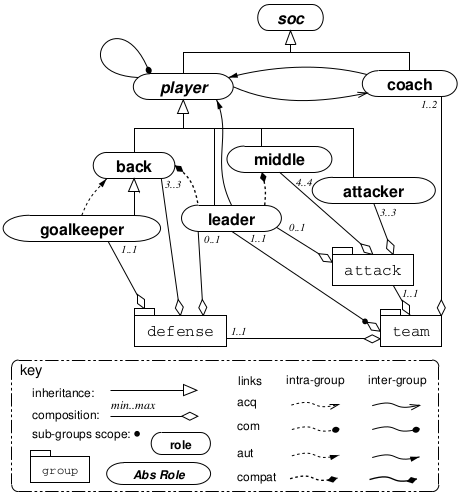
\includegraphics[width=0.7\textwidth]{figures/soccer_ss.png}
                \caption*{Structural Specifications}
            \end{figure}
        \end{column}
        \hspace{-20ex}
        \begin{column}{0.5\textwidth}
            \centering
            \begin{figure}[H]
                \centering
                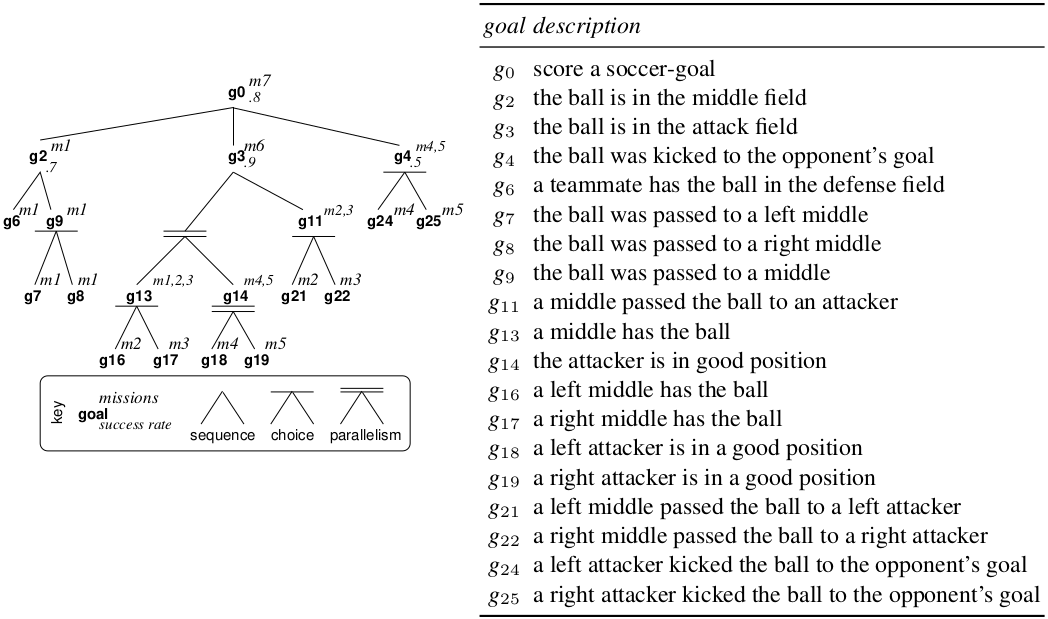
\includegraphics[width=1.2\textwidth]{figures/soccer_fs.png}
                \caption*{Functional Specifications}
            \end{figure}
        \end{column}
    \end{columns}

    \ \\

    \begin{minipage}{\textwidth}
        \centering
        \begin{figure}[H]
            \centering
            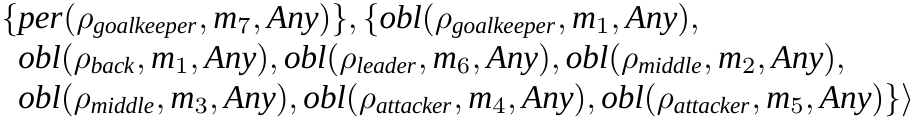
\includegraphics[width=0.4\linewidth]{figures/soccer_ds.png}
            \caption*{Deontic Specifications}
        \end{figure}
    \end{minipage}

\end{frame}

\begin{frame}{Appendix}{Q: Do organizational constraints harm exploration?}
    \begin{itemize}
        \item \textbf{Not necessarily.} Constraints can actually \textit{guide exploration} more effectively by pruning unpromising behaviors.
        \item The hardness parameter allows tuning how strictly agents follow roles/goals.
        \item With soft constraints, agents retain exploration capabilities while being nudged toward structured behaviors.
    \end{itemize}
\end{frame}

\begin{frame}{Appendix}{Q: How is MOISE+MARL different from Hierarchical RL?}
    \begin{itemize}
        \item HRL decomposes tasks internally via learned hierarchies.
        \item MOISE+MARL imposes external \textbf{organizational roles and missions} as behavioral constraints.
        \item Roles are \textit{interpretable, configurable, and decoupled from the agent architecture}.
    \end{itemize}
\end{frame}

\begin{frame}{Appendix}{Q: Does your framework scale with many agents? What about policy plasticity?}
    \begin{itemize}
        \item Scalability: Roles can be \textbf{abstract} and applied to groups of agents (e.g., “defender”, “collector”).
        \item Plasticity: Constraint strength is tunable. Soft constraints preserve policy adaptability.
        \item Trade-off: Strong constraints yield stability, soft ones allow flexibility.
    \end{itemize}
\end{frame}

\begin{frame}{Appendix}{Q: How does MOISE+MARL handle partial observability?}
    \begin{itemize}
        \item Built on the Dec-POMDP formalism: partial observability is natively supported.
        \item Constraints apply to agents' \textbf{observed trajectories}—not full states.
        \item No need for global knowledge or central control.
    \end{itemize}
\end{frame}

\begin{frame}{Appendix}{Q: Is the TEMM method computationally heavy? Can it generalize?}
    \begin{itemize}
        \item TEMM is applied post-training. It uses clustering (K-means, hierarchical) and can be parallelized.
        \item It supports any environment with labeled trajectories and does not depend on the training algorithm.
        \item Currently offline only; real-time extensions are under consideration.
    \end{itemize}
\end{frame}

\begin{frame}{Appendix}{Q: How do you evaluate the impact of organizational constraints?}
    \begin{itemize}
        \item We compare a Reference Baseline (no constraints) and a Constrained Baseline (MOISE+MARL).
        \item Metrics: Cumulative Reward, Convergence Rate, Org. Fit, Consistency, Robustness, Violation Rate.
        \item MOISE+MARL consistently improves organizational fit and stability across all environments tested.
    \end{itemize}
\end{frame}

% ===============

\begin{frame}{Appendix}
    {Context}

    \begin{block}{Multi-Agent Systems (MAS) paradigm for complex \& distributed problems}
        \begin{itemize}
            \item \textbf{task decomposition}: missions delegated to agents achieved through cooperation~\parencite{Raileanu2023};
            \item \textbf{benefits}: handle conflicting goals, parallel computation, system robustness, scalability\dots
        \end{itemize}
    \end{block}

    \begin{block}{\textbf{Organization}: key for MAS designing}
        \begin{itemize}
            \item \textbf{coordination}: how to collaboratively achieve a common goal~\parencite{Hubner2007};
            \item \textbf{dynamic \& uncertain environments}: flexible runtime behavior to adapt~\parencite{Kathleen2020};
        \end{itemize}
    \end{block}

    \begin{block}{Methods and practice for MAS design}
        \begin{itemize}
            \item \textbf{approach + organizational model}: methods rely on designers' experience to hand-craft agents' \textbf{policies} so resulting MAS achieve goals;
                  %   \begin{itemize}
                  %       \item Examples: \emph{GAIA}~\parencite{Wooldridge2000,Cernuzzi2014}, \emph{ADELFE}~\parencite{Mefteh2015}, or \emph{DIAMOND}~\parencite{Jamont2015}, \emph{KB-ORG}~\parencite{Sims2008}
                  %   \end{itemize}
            \item \textbf{simulation to reality}: 1) safe \& efficient MAS design in high fidelity simulated environment; \quad 2) transfer to real environment to perform adequately~\parencite{Schon2021}.
        \end{itemize}
        \quad $\Longrightarrow$ \textbf{Iterative process proceeding by trial and error}

    \end{block}

\end{frame}

\begin{frame}{Appendix}{CAGE Challenge 3}
    \begin{figure}
        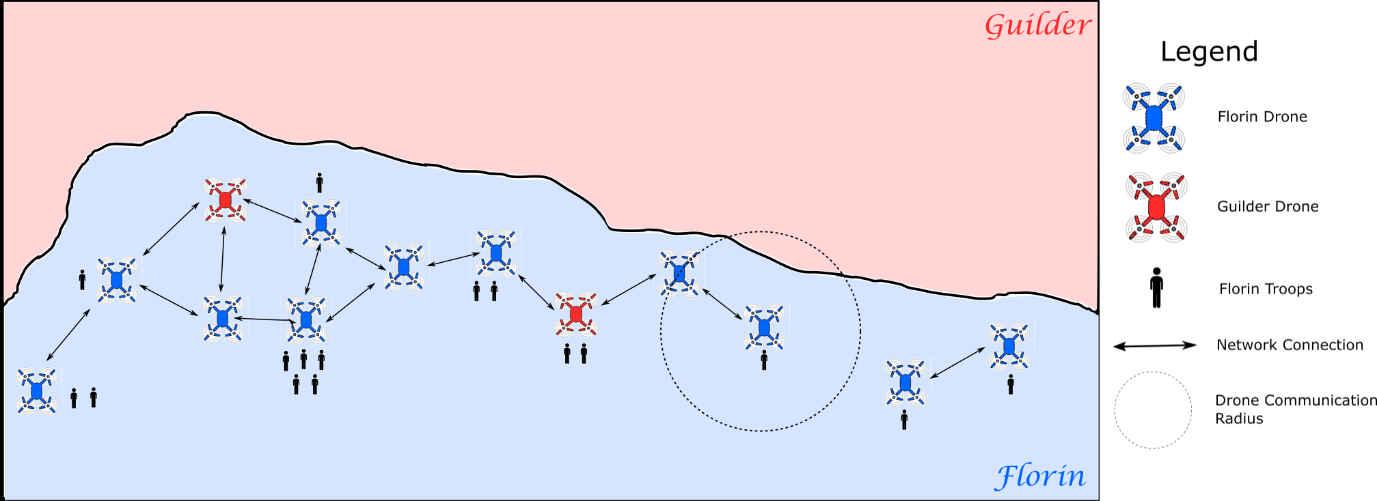
\includegraphics[width=0.9\linewidth]{figures/cage_challenge_3.png}
        \caption*{Florin forces patrolling the Guilder border with troops that communicate via an ad-hoc network provided by aerial drones. Here, Guilder has successfully corrupted two drones within this network and can thus intercept, or alter, some of the messages being communicated.}
    \end{figure}
\end{frame}

\begin{frame}{Appendix}{Prey-predator}
    \begin{figure}
        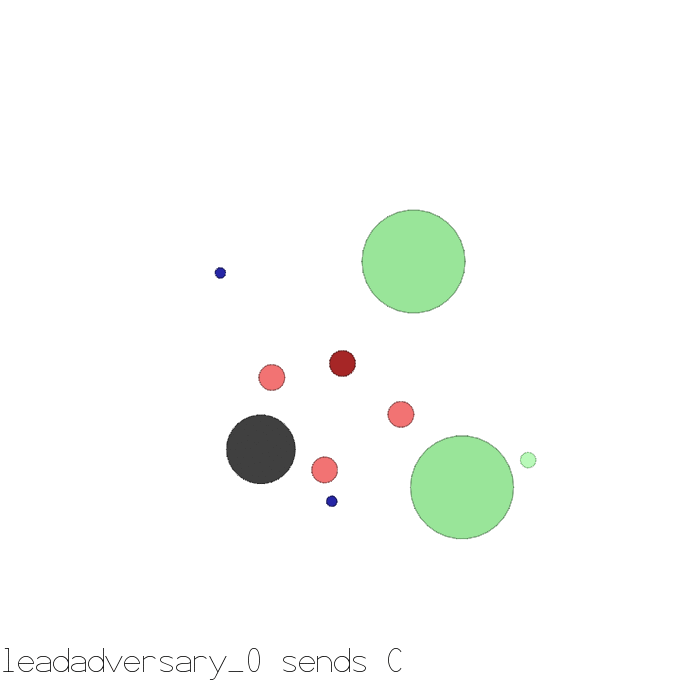
\includegraphics[width=0.5\linewidth]{figures/mpe_simple_world_comm.png}
    \end{figure}
\end{frame}

\begin{frame}{Appendix}{Knight, archers, zombies}
    \begin{figure}
        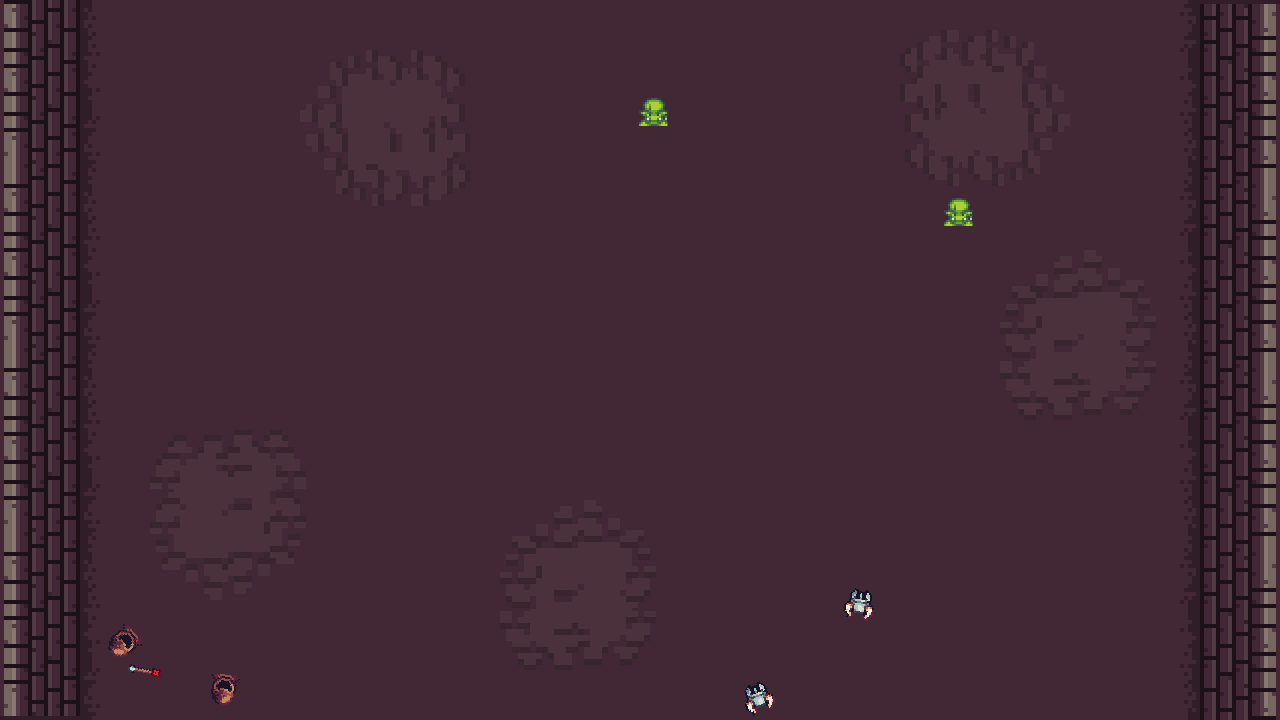
\includegraphics[width=0.8\linewidth]{figures/butterfly_knights_archers_zombies.png}
    \end{figure}
\end{frame}

\begin{frame}{Appendix}
    {MAS basics}

    \begin{block}{Keywords}
        \begin{itemize}
            \item \textbf{Agent}: entity immersed in an environment perceiving observation and making decision autonomously to achieve some goals;
            \item \textbf{MAS}: a set of agents collaborating with self/re-organizing mechanisms to achieve their goal;
            \item \textbf{Organization}: the agents' interactions even though it may be implicit;
            \item \textbf{Organizational Model (OM)}: medium to formally describe an explicit/implicit organization;
            \item \textbf{Organizational Specifications (OS)}: components of an OM to characterize an organization
        \end{itemize}
    \end{block}

    \begin{block}{Organizational model: $\mathcal{M}OISE^+$}
        \begin{itemize}
            \item more complex than \emph{Agent Group Roles} (integration of standards);
            \item takes into account the social aspects between agents explicitly;
            \item possible to link agents' policies to organizational specifications.
        \end{itemize}
    \end{block}

\end{frame}

\begin{frame}{Appendix}
    {MARL basics}

    \begin{block}{Keywords}
        \begin{itemize}
            \item \textbf{Policy}: the \textquote{logic} to choose next action according to observation for an agent;
            \item \textbf{History/trajectory}: the tuple of (observation, action) couples over an episode;
            \item \textbf{Joint-policy / Joint-history}: all of the agents' policies / histories as tuples;
            \item \textbf{Reinforcement learning}: an agent updates its policy to maximize a cumulative reward;
            \item \textbf{Multi-Agent Reinforcement Learning (MARL)}: extends to multiple agents that learn while considering the actions of other agents;
        \end{itemize}
    \end{block}

\end{frame}

\begin{frame}{Appendix}{AOMEA approach: Overview}

    \begin{columns}

        \begin{column}{0.6\textwidth}

            \textbf{Phase 1: Modeling}

            \begin{itemize}
                \item Manually develop a simulated environment ($1.1$) where agents must cooperate to achieve goal ($1.2$);
                \item Can define expected roles behavior as histories;
                \item May constraint agents to roles ($1.3$).
            \end{itemize}

        \end{column}

        \begin{column}{0.4\textwidth}
            \centering
            \adjustbox{trim={0.\width} {0.82\height} {0.\width} {0.\height}, clip}{%
                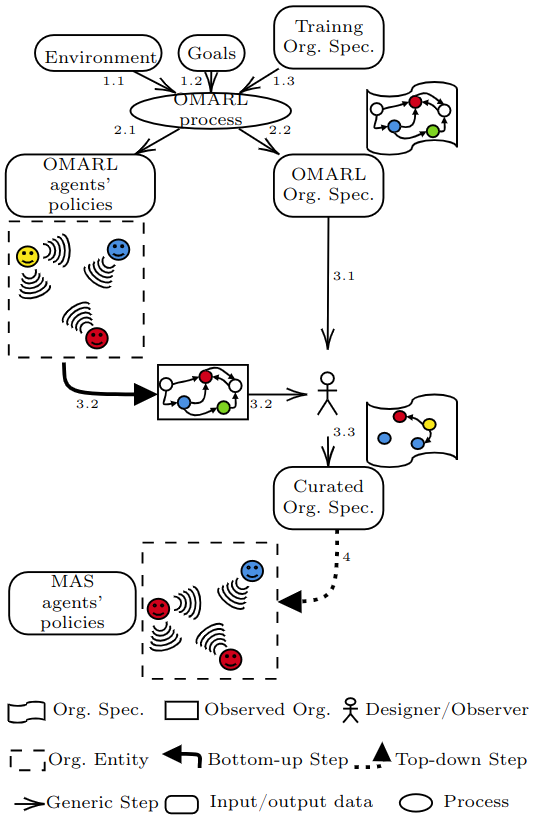
\includegraphics[width=1.2\linewidth]{figures/AOMEA_illustrative_view}
            }
        \end{column}

    \end{columns}

\end{frame}


\begin{frame}{Appendix}{AOMEA approach: Overview}

    \begin{columns}

        \begin{column}{0.6\textwidth}

            \textbf{Phase 2: Solving}

            \begin{itemize}
                \item Organization-oriented MARL (OMARL) algorithm: MARL process augmented with Organizational model;
                \item Solve satisfying constrained roles' histories ($2.1$);
                \item Gets associated OS ($2.2$)
            \end{itemize}

        \end{column}

        \begin{column}{0.4\textwidth}
            \centering
            \adjustbox{trim={0.\width} {0.56\height} {0.\width} {0.\height}, clip}{%
                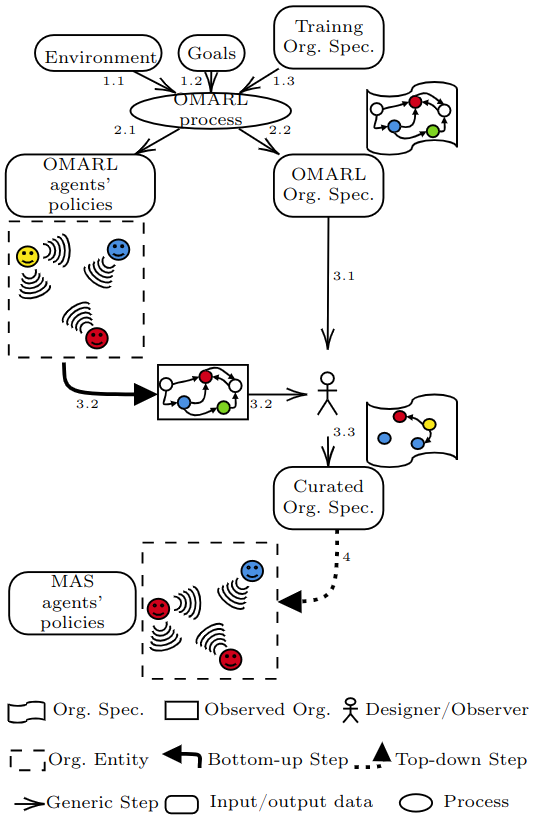
\includegraphics[width=1.2\linewidth]{figures/AOMEA_illustrative_view}
            }
        \end{column}

    \end{columns}


\end{frame}

\begin{frame}{Appendix}{AOMEA approach: Overview}

    \begin{columns}

        \begin{column}{0.6\textwidth}

            \textbf{Phase 3: Analyzing}

            \begin{itemize}
                \item Designers observe the trained agents' policies ($3.2$);
                \item Designers observe the computed OS ($3.1$): understand how they reach the goal;
                \item Designers get some design indications for a MAS to achieve the goal: curated OS ($3.3$).
            \end{itemize}


        \end{column}

        \begin{column}{0.4\textwidth}
            \centering
            \adjustbox{trim={0.\width} {0.35\height} {0.\width} {0.188\height}, clip}{%
                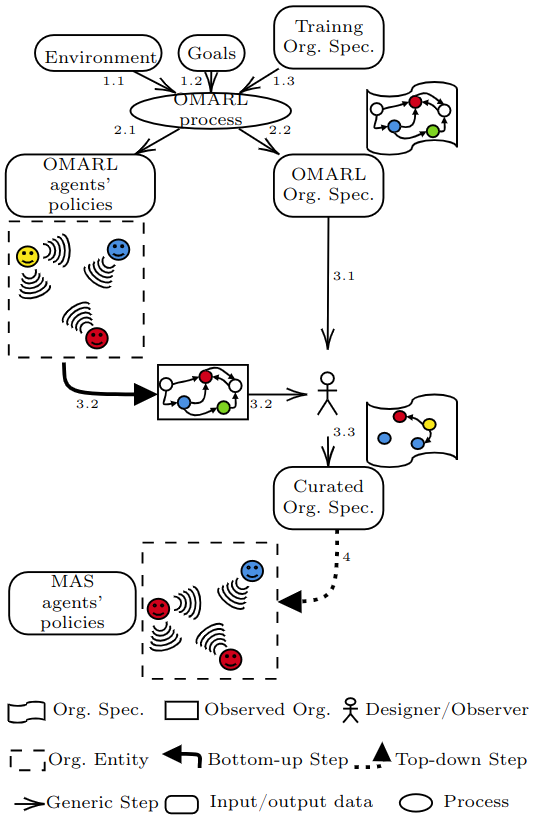
\includegraphics[width=1.2\linewidth]{figures/AOMEA_illustrative_view}
            }
        \end{column}

    \end{columns}

\end{frame}

\begin{frame}{Appendix}{AOMEA approach: Overview}

    \begin{columns}

        \begin{column}{0.6\textwidth}

            \textbf{Phase 4: Developing}

            \begin{itemize}
                \item Designers observe the curated OS for implementing a MAS;
                \item Regular MAS development hence addressing safety issues;
                \item Implemented MAS assessed in simulations.
            \end{itemize}

        \end{column}

        \begin{column}{0.4\textwidth}
            \centering
            \adjustbox{trim={0.\width} {0.15\height} {0.\width} {0.57\height}, clip}{%
                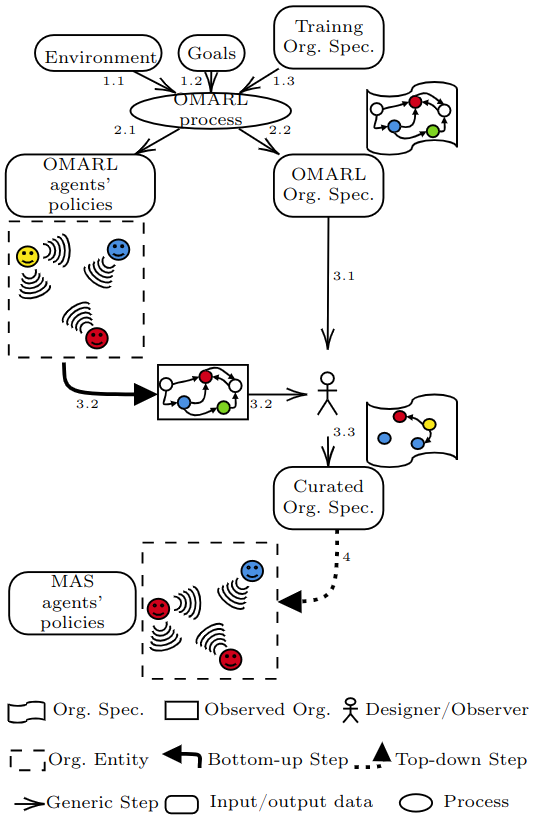
\includegraphics[width=1.2\linewidth]{figures/AOMEA_illustrative_view}
            }
        \end{column}

    \end{columns}

\end{frame}



\begin{frame}{Appendix}{AOMEA approach: Theoretical core}

    \begin{block}{Organization-oriented MARL (OMARL)}
        An MARL process augmented with an OM for:
        \begin{itemize}
            \item \textbf{Constraining Policies Space}: gets the joint-policies satisfying the given design specifications;
            \item \textbf{Inferring Organizational Specifications}: gets the specifications from the agents' policies.
        \end{itemize}

    \end{block}

    \begin{block}{\emph{Partial Relations with Agent History and Organization Model} algorithm (PRAHOM)}
        Implementing an OMARL process\dots
        \begin{enumerate}
            \item \textbf{Constraining Policies Space}
                  \begin{itemize}
                      \item Cannot use policies directly $\rightarrow$ \textbf{histories} characterizing \textbf{policies};
                      \item Relations between \textbf{OS} to expected \textbf{histories};
                      \item Agents constrained to OS $\rightarrow$ at each step: available actions updated regarding \textbf{OS} histories.
                  \end{itemize}

            \item \textbf{Inferring Organizational Specifications}
                  \begin{itemize}
                      \item Analyze histories $\rightarrow$ characterize collective behaviors as OS;
                      \item Using known relations between OS and histories;
                      \item Using general OS definition regarding histories.
                  \end{itemize}
        \end{enumerate}
    \end{block}
\end{frame}

\begin{frame}{Appendix}{AOMEA approach: Theoretical core}

    \textbf{Constraining Policies Space} during training

    \begin{columns}

        \begin{column}{0.3\textwidth}

            \begin{itemize}
                \item At each step, available actions set is changed to match policy constraints defined by users;
                \item Constraints integrated through: external correction, learning, internal policy change.
            \end{itemize}

        \end{column}

        \begin{column}{0.8\textwidth}
            \begin{figure}
                \centering
                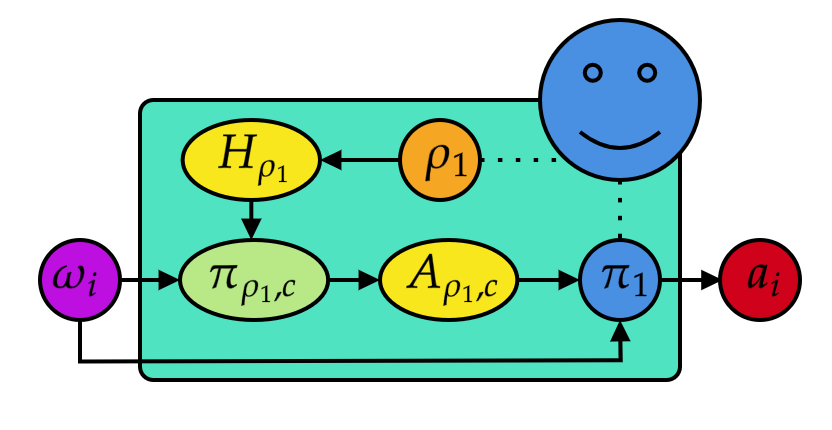
\includegraphics[width=0.7\linewidth]{figures/prahom_training_constrain.png}
                \caption*{A summary view of the PRAHOM constraining}
                \label{fig:prahom_process}
            \end{figure}
        \end{column}

    \end{columns}

\end{frame}


\begin{frame}{Appendix}{AOMEA approach: Theoretical core}

    \textbf{Inferring Organizational Specifications}

    \begin{columns}

        \begin{column}{0.3\textwidth}

            \begin{itemize}
                \item \textbf{Knowledge-based Organizational Specifications Identification (KOSIA)}
                \item \textbf{General Organizational Specifications Infererence (GOSIA)}
            \end{itemize}

        \end{column}

        \begin{column}{0.8\textwidth}
            \begin{figure}
                \centering
                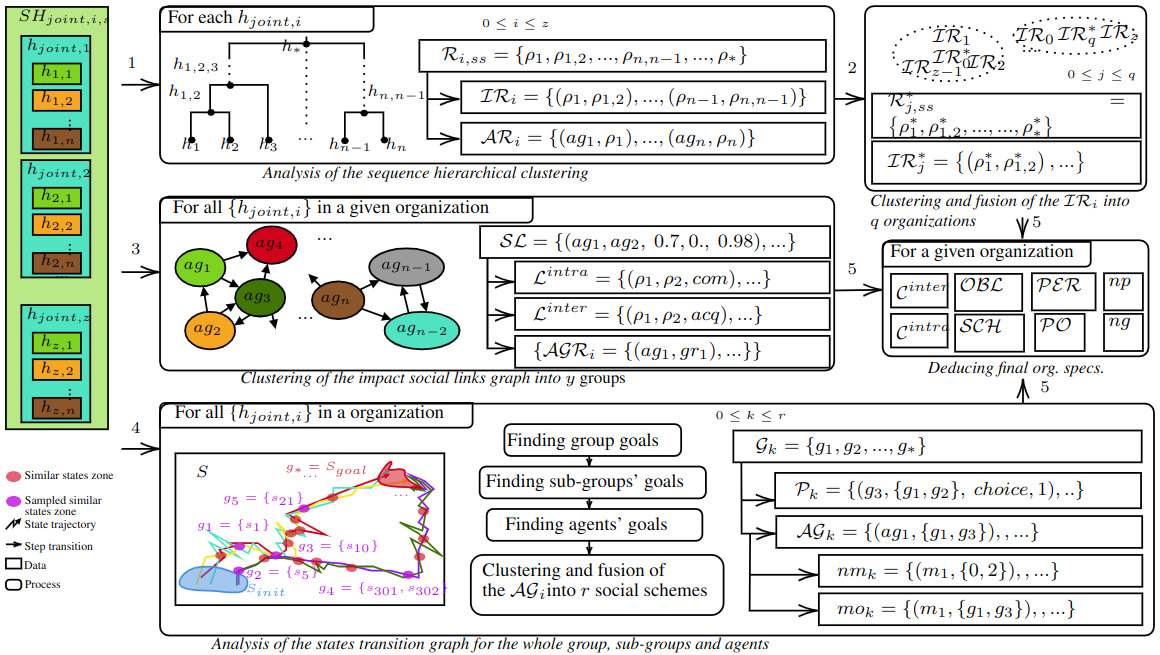
\includegraphics[width=0.95\linewidth]{figures/GOSIA_view.png}
                \caption*{A summary view of the GOSIA process}
                \label{fig:gosia_process}
            \end{figure}
        \end{column}

    \end{columns}

\end{frame}


\begin{frame}{Appendix}{Constrained Reinforcement Learning (Constrained-RL)}

    \begin{itemize}
        \item Learn a policy that optimizes reward while respecting \textbf{safety} or \textbf{performance} constraints.

        \item \textbf{Hard constraints}: must always be respected (e.g., shielding).
        \item \textbf{Soft constraints}: enforced on average or via penalties.

        \item \textbf{Main methods:}
              \begin{itemize}
                  \item \textbf{Reward Shaping}: add penalties when constraints are violated.
                  \item \textbf{Policy Projection}: adjust actions to remain within limits.
                  \item \textbf{Dual Variables}: use Lagrangian multipliers to manage constraints.
              \end{itemize}

    \end{itemize}
\end{frame}

\begin{frame}{Appendix}{Safe Exploration and Shielding in Reinforcement Learning}

    \begin{itemize}
        \item \textbf{Safe Exploration} $\rightarrow$ ensure safety during exploration by limiting risky behaviors.
        \item Mainly by modifying the reward function (e.g., via Lagrangian), but also with:
        \item \textbf{Shielding}: intervene in real time to block unsafe actions and ensure safe exploration.
    \end{itemize}

    \textbf{Reference:} \\
    \textit{Akifumi Wachi, Wataru Hashimoto, Xun Shen, \& Kazumune Hashimoto (2023). Safe Exploration in Reinforcement Learning: A Generalized Formulation and Algorithms. In NeurIPS 2023.}

\end{frame}

\begin{frame}[fragile]{Appendix}{Optuna Usage Example}
    \begin{itemize}
        \item \textbf{Optuna} is an open-source library for hyperparameter optimization (HPO), widely used in machine learning.
        \item Examples of hyperparameters: learning rate, activation function, number of layers, layer sizes, distance threshold for clustering, etc.
        \item \textbf{Steps to use Optuna:}
              \begin{itemize}
                  \item \texttt{1.} Define an objective function.
                  \item \texttt{2.} Launch a study with Optuna.
                  \item \texttt{3.} Use the best result to train the model.
              \end{itemize}
    \end{itemize}

    \begin{lstlisting}[language=Python, basicstyle=\small\ttfamily, frame=single, caption=Optuna example in Python]
import optuna

def objective(trial):
    x = trial.suggest_float("x", -10, 10)
    return (x - 2) ** 2  # Mock value function

study = optuna.create_study(direction="minimize")
study.optimize(objective, n_trials=100)

print(study.best_params)  # Display best parameters
    \end{lstlisting}
\end{frame}

\begin{frame}{Appendix}{PettingZoo Overview}
    \begin{itemize}
        \item Python library for multi-agent environments.
        \item Simplifies training and evaluation of agents in various multi-agent setups.
        \item \textbf{Main features:}
              \begin{itemize}
                  \item Supports multiple environment types (turn-based, parallel, etc.).
                  \item Easy integration with RL frameworks like RLlib.
                  \item Compatible with Gym APIs for intuitive usage.
              \end{itemize}
        \item \textbf{Example environments included:}
              \begin{itemize}
                  \item Games: \textit{TicTacToe}, \textit{ConnectFour}
                  \item Collaboration/competition: \textit{Pistonball}, \textit{Prisoner's Dilemma}
                  \item Integration with Atari multi-agent suite
              \end{itemize}
    \end{itemize}
\end{frame}

\begin{frame}[fragile]{Appendix}{PettingZoo Usage Example}
    \begin{itemize}
        \item Example: Create and interact with an environment.
        \item Load environment, reset, and interact step-by-step with agents.
    \end{itemize}
    \vspace{0.3cm}
    \begin{lstlisting}[language=Python, basicstyle=\ttfamily\small]
from pettingzoo.butterfly import pistonball_v6

# Create and reset environment
env = pistonball_v6.env()
env.reset()

# Interaction loop
for agent in env.agent_iter():
    obs, reward, done, info = env.last()
    action = env.action_space(agent).sample()  # Random action
    env.step(action)
    if done:
        env.reset()  # Reset if episode is finished
    \end{lstlisting}
\end{frame}

\begin{frame}{Appendix}{KB-Org}
    \frametitle{Organization-based Multi-Agent Systems: From Modeling to Implementation}

    \begin{itemize}
        \item Models and implements organization-based MAS;
        \item Embeds organizational concepts to structure agent behavior and interactions;
        \item Provides a repository of ready-to-use organizational templates;
        \item Aims at improving explainability and coordination.
    \end{itemize}

    \vspace{1em}
    Sims, V. (2008). Automated organization design for multi-agent systems. Autonomous Agents and Multi-Agent Systems, 16(2), 151–185.

\end{frame}

\begin{frame}{Appendix}{MARLlib Overview}

    \begin{itemize}
        \item Python library for MARL
        \item Supports various environments: PettingZoo, StarCraft II, MPE, etc.
        \item Implements multiple MARL algorithms: MADDPG, MAPPO, etc.
        \item Offers tools for training, evaluation, and algorithm comparison.
        \item Provides fine-tuned configuration presets for many environments.
    \end{itemize}

\end{frame}

\begin{frame}[allowframebreaks]{Appendix}{MARLlib Algorithms Overview}

    \begin{itemize}
        \item \textbf{Value-Based Algorithms}
              \begin{itemize}
                  \item \textbf{Multi-Agent Q-Learning}: Basic multi-agent extension of Q-learning.\newline
                  \textit{Note: Simple but suffers from scalability and non-stationarity issues.}
                  \item \textbf{MADDPG}: Extension of DDPG for MARL.\newline
                  \textit{Note: Suitable for continuous actions but data-hungry and complex.}
              \end{itemize}

        \item \textbf{Policy-Based Algorithms}
              \begin{itemize}
                  \item \textbf{REINFORCE}: Basic policy gradient method for direct policy learning.\newline
                  \textit{Note: Works in stochastic environments but has high variance.}
                  \item \textbf{MAPPO (Multi-Agent PPO)}: Multi-agent extension of PPO.\newline
                  \textit{Note: Stabilizes updates, but requires tuning and high compute.}
              \end{itemize}

        \item \textbf{Hybrid Algorithms}
              \begin{itemize}
                  \item \textbf{A3C}: Combines value and policy learning for balanced exploration.\newline
                  \textit{Note: Fast training but needs complex synchronization.}
                  \item \textbf{MAPPO}: PPO-based hybrid with centralized training.\newline
                  \textit{Note: Effective for cooperative tasks, but resource-intensive.}
              \end{itemize}

        \item \textbf{Theoretical and Game-Based Algorithms}
              \begin{itemize}
                  \item \textbf{IQL (Independent Q-Learning)}: Per-agent Q-learning.\newline
                  \textit{Note: Easy to implement but suffers from non-stationarity.}
                  \item \textbf{COMA}: Uses counterfactual baselines to assess agent contributions.\newline
                  \textit{Note: Reduces variance, improves cooperation, but computationally heavy.}
              \end{itemize}

        \item \textbf{Centralized Training with Decentralized Execution (CTDE)}
              \begin{itemize}
                  \item \textbf{QMIX}: Decomposes Q-values to support coordination.\newline
                  \textit{Note: Balances centralized learning and decentralized execution.}
                  \item \textbf{VDN (Value Decomposition Networks)}: Simplifies coordination via value decomposition.\newline
                  \textit{Note: Efficient, but limited for complex interactions.}
              \end{itemize}
    \end{itemize}

\end{frame}
